\documentclass{kththesis}
\usepackage[utf8]{inputenc}
%\usepackage[pdftex]{graphicx}
\usepackage{amsmath}
\usepackage{amsthm}
\usepackage{amsfonts}
\usepackage{amssymb}
\usepackage[hyphens]{url}
\usepackage{hyperref}
\usepackage{siunitx}
\usepackage{pdflscape}
\usepackage{geometry}
\usepackage[toc]{glossaries} % https://www.overleaf.com/learn/latex/Glossaries
\usepackage{parskip} % empty line between paragraphs
\usepackage[textwidth=2cm]{todonotes}
\usepackage{listings}
\usepackage{float}
\usepackage{pmboxdraw}
\usepackage{textcomp} % for the apostrophe

% hyperref setup
\definecolor{darkgreen}{RGB}{0,180,0}
\hypersetup{
    colorlinks = true,
    linkbordercolor = {white},
    linkcolor = red,
    anchorcolor = black,
    citecolor = darkgreen,
    filecolor = cyan,
    menucolor = black,
    runcolor = cyan,
    urlcolor = magenta
}

% Bib setup
\usepackage{csquotes} % Recommended by biblatex
\usepackage[style=numeric,sorting=none,backend=biber]{biblatex}
\addbibresource{references.bib} % The file containing our references, in BibTeX format

\title{Experiments on automation of formal verification of devices at the binary level}
%\alttitle{}
\author{Thomas Lacroix}
\email{thomas.lacroix@insa-lyon.fr}
\supervisor{Mads Dam}
\examiner{TODO}
\hostcompany{Division of Theoretical Computer Science - KTH}
\programme{Master in Computer Science}
\school{Computer Science department - INSA Lyon}
\date{\today}

% Uncomment the next line to include cover generated at https://intra.kth.se/kth-cover?l=en
% \kthcover{kth-cover.pdf}

%%%%%%%%%%%%%%%%%%%%%%%%%%%%%%%%%%%%%%%%%%%%%%%%%%%%%%%%%%%%%%%%%%%%%%%%%%%%%%%%%%%%%%%%
%%%%%%%%%%%%%%%%%%%%%%%%%%%%%%%%%%%%%%%%%%%%%%%%%%%%%%%%%%%%%%%%%%%%%%%%%%%%%%%%%%%%%%%%
%% Glossary

\renewcommand*{\glstextformat}[1]{\textcolor{black}{\textbf{#1}}}

\makeglossaries

%\gls{latex} or \Gls{latex}, \Glspl{formula}
%\acrlong{gcd} \acrshort{gcd} \acrfull{gcd}

\newglossaryentry{FreeRTOS} {
    name={FreeRTOS},
    description={FreeRTOS is a free and open-source market leading real time operating system for microcontrollers and small microprocessors. Website: \url{https://freertos.org/}}
}
\newglossaryentry{iot} {
    name={IoT},
    description={Internet Of Things. This is the idea of connecting every devices---such that temperature sensors, lamps, video cameras or wearable devices---to the Internet}
}
\newacronym{prosper}{PROSPER}{Provably Secure Execution Platforms for Embedded Systems}
\newglossaryentry{transpilation} {
    name={transpilation},
    description={Process carried-out by a \gls{transpiler}}
}
\newglossaryentry{transpiler} {
    name={transpiler},
    description={A transpiler, or source-to-source compiler, is a compiler that takes source code written in a programming language A, and producing an equivalent source code in a programming language B. A and B can be different languages or the same. They differ from traditional compilers in that compilers generally produce machine code}
}
\newglossaryentry{proof-producing} {
    name={proof-producing},
    description={A proof-producing analysis or procedure is a procedure that yields its result in the form of a formal proof. Therefore, those procedures represent the highest degree possible of trustworthiness. However, great care must be taken to ensure that the definitions used to phrase the proof are sound and actually represent the properties to be proved. Moreover, implementing proof-producing code is costly and thus should be used with discernment}
}
\newacronym{holba}{HolBA}{HOL4 Binary Analysis Platform}
\newacronym{bap}{CMU BAP}{Carnegie Mellon University Binary Analysis Platform}
\newglossaryentry{BIR} {
    name={BIR},
    description={\acrshort{holba}'s machine-independent binary intermediate representation}
}
\newglossaryentry{BSL} {
    name={BSL},
    description={BIR Simple Language. It is also a word play with DSL which means Domain Specific Language}
}
\newacronym{ISA}{ISA}{Instruction Set Architecture}
\newacronym{SMT}{SMT}{Satisfiability Modulo Theories}
\newacronym{SAT}{SAT}{Boolean SATisfiability Problem}
\newacronym{NIC}{NIC}{Network Interface Controller}
\newacronym{CFG}{CFG}{Control Flow Graph}
\newacronym{SML}{SML}{Standard ML}
\newacronym{IR}{IR}{Intermediate Representation}

%% End of Glossary
%%%%%%%%%%%%%%%%%%%%%%%%%%%%%%%%%%%%%%%%%%%%%%%%%%%%%%%%%%%%%%%%%%%%%%%%%%%%%%%%%%%%%%%%
%%%%%%%%%%%%%%%%%%%%%%%%%%%%%%%%%%%%%%%%%%%%%%%%%%%%%%%%%%%%%%%%%%%%%%%%%%%%%%%%%%%%%%%%

%%%%%%%%%%%%%%%%%%%%%%%%%%%%%%%%%%%%%%%%%%%%%%%%%%%%%%%%%%%%%%%%%%%%%%%%%%%%%%%%%%%%%%%%
%%%%%%%%%%%%%%%%%%%%%%%%%%%%%%%%%%%%%%%%%%%%%%%%%%%%%%%%%%%%%%%%%%%%%%%%%%%%%%%%%%%%%%%%
%% Some macros

\newcommand{\htriple}[3]{\ensuremath{\{#1\}~#2~\{#3\}}}
\newcommand{\WP}{\ensuremath{\mathit{WP}}}
\newcommand{\notimplies}{%
  \mathrel{{\ooalign{\hidewidth$\not\phantom{=}$\hidewidth\cr$\implies$}}}}
\newcommand{\eqdef}{\stackrel{def}{=}}
\newcommand{\eqeval}{\stackrel{eval}{=}}

%\newtheorem{eq_theorem}{Theorem}[section]
%\numberwithin{equation}{eq_theorem}
%
%\newtheorem{eq_lemma}{Lemma}[section]
%\numberwithin{equation}{eq_lemma}

\newtheorem{theorem}{Theorem}[section]
\newtheorem{corollary}{Corollary}[theorem]
\newtheorem{lemma}[theorem]{Lemma}
\newtheorem{remark}{Remark}
\newtheorem*{remark*}{Remark}

%% Listing settings

\definecolor{codegreen}{rgb}{0,0.6,0}
\definecolor{codegray}{rgb}{0.5,0.5,0.5}
\definecolor{codepurple}{rgb}{0.58,0,0.82}
\definecolor{codeblue}{rgb}{0.10,0,0.82}
\definecolor{codebackcolour}{rgb}{0.95,0.95,0.92}
 
%% End of macros
%%%%%%%%%%%%%%%%%%%%%%%%%%%%%%%%%%%%%%%%%%%%%%%%%%%%%%%%%%%%%%%%%%%%%%%%%%%%%%%%%%%%%%%%
%%%%%%%%%%%%%%%%%%%%%%%%%%%%%%%%%%%%%%%%%%%%%%%%%%%%%%%%%%%%%%%%%%%%%%%%%%%%%%%%%%%%%%%%

\begin{document}

\frontmatter % titlepage, abstracts and TOC

\titlepage

\begin{abstract}
  With the advent of virtualization, more and more work is put into the verification of hypervisors. Being low level softwares, such verification should preferably be performed at binary level. Binary analysis platforms are being developed to help perform these proofs, but a lot of the work has to be carried out manually.

  In this thesis, we focus on the formal verification of a Network Interface Controller (NIC), more specifically we look at how to automate and reduce the boilerplate work from an existing proof. We base our work on the HolBA platform, its hardware-independent intermediate representation language BIR and supporting tools, and we experiment on how to perform this proof by leveraging existing tools.

  We first replaced the existing NIC model written in HOL4 to an equivalent one written using BIR, enabling the use of HolBA tools. Secondly, we developed some visualization tools to help navigate and gain some insight in the existing proof and its structure. Thirdly, we experimented with the use of Hoare triples in conjunction with an SMT solver to perform contract verification. Finally, we proved a simple contract written in terms of the formal NIC model on the BIR implementation of this model, unlocking the way of performing more complex proofs using the HolBA platform.

  \textit{Keywords}: binary analysis, formal verification, proof producing analysis, theorem proving
\end{abstract}

%\begin{otherlanguage}{swedish}
%  \begin{abstract}
%  \end{abstract}
%\end{otherlanguage}
\begin{otherlanguage}{french}
  \begin{abstract}
    Avec la démocratisation de la virtualisation, de plus en plus d'efforts sont consacrés à la vérification des hyperviseurs. S'agissant de logiciels de bas niveau, une telle vérification devrait de préférence être effectuée au niveau binaire. Des plates-formes d'analyse binaire sont en cours de développement pour aider à réaliser ces preuves, mais une grande partie du travail doit encore être effectuée manuellement.

    Dans cette thèse, nous nous concentrons sur la vérification formelle d'un Contrôleur d'Interface Réseau (NIC), plus spécifiquement sur la manière d'automatiser et de réduire le travail répétitif d'une preuve existante. Nous nous basons sur la plate-forme HolBA, son langage de représentation intermédiaire indépendant du matériel, BIR et ses outils de support, et nous nous intéressons à la manière de réaliser cette preuve en utilisant des outils existants.

    Nous avons d'abord remplacé le modèle NIC existant écrit en HOL4 par un modèle équivalent écrit en BIR, permettant ainsi l'utilisation des outils de HolBA. Deuxièmement, nous avons développé des outils de visualisation pour nous aider à naviguer et à mieux comprendre la preuve existante et sa structure. Troisièmement, nous avons expérimenté l'utilisation des triplets de Hoare en conjonction avec un solveur SMT pour effectuer une vérification par contrat. Enfin, nous avons prouvé un contrat simple écrit en termes du modèle formel du NIC sur l'implémentation de ce modèle en BIR, ouvrant la voie à la réalisation de preuves plus complexes avec la plate-forme HolBA.

    \textit{Mot-clés} : binary analysis, formal verification, proof producing analysis, theorem proving
  \end{abstract}
\end{otherlanguage}

\listoftodos
\todo{Include:%
a) Git workflow for a team;%
b) LogLib (and tracing in general); -> annex%
c) CI to track regressions + static analysis;%
d) Simple interface for CFG lib;%
e) Mention the "while 1: automaton.step()";%
}

\tableofcontents

\printglossaries

\mainmatter % Thesis content

\chapter{Introduction}
\vspace{-1cm}
\textit{This chapter serves as an introduction to the degree project and presents the background of the work along with this thesis objective. Delimitations to the project and the choice of methodology are also discussed.}

\section{Background}

Embedded systems are becoming more and more common with the current advent of \Gls{iot} and mobile computing platforms such as smartphones. Those systems are fully-fledged computers with powerful hardware, complete operating systems and access to Internet. Such systems can run security-critical services, such as a building security system or automatic toll gates, or carry valuable information as it is the case for personal smartphones. Therefore, these two characteristics make them targets of choice for attackers.

The \gls{prosper} project \cite{noauthor_prosper:_nodate} aims to develop a secure and formally verified hypervisor for embedded systems. Hypervisors are thin layers running directly on top of hardware providing the ability to run virtualized applications, such that operating systems or realtime control systems. Those virtualized applications then don't have privileged access to the hardware and have to go through the hypervisor. This allows different applications to share the same hardware while providing strong isolation between them, thus ensuring confidentiality and security. Moreover, security not only means protection from external attacks, but also resilience to bugs. If multiple critical systems are running on the same hardware, bugs or crashes in some systems shouldn't affect the others from behaving correctly. Figure \ref{figure-hypervisor-simple} shows a system running two isolated Linux on top of a hypervisor.

\begin{figure}[ht]
	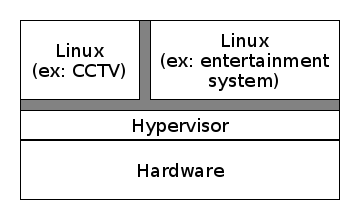
\includegraphics[height=4cm]{figures/figure-hypervisor-simple.png}
	\centering
	\caption{Two Linux on top of an hypervisor. They run isolated from each other and from the hypervisor.}
	\label{figure-hypervisor-simple}
\end{figure}

Previous work in the \acrshort{prosper} project achieved \cite{noauthor_prosper:_nodate-1} to formally verify a simple separation kernel \cite{dam_formal_2013}, which later resulted into an implementation of a working hypervisor. Then, they achieved to run both Linux and \gls{FreeRTOS} on top of it. Finally, they formally verified memory isolation for virtualized applications \cite{nemati_trustworthy_2015}. Now, among other projects, the PROSPER team is working on device virtualization, allowing to give access to hardware devices to virtualized applications. An interesting example are \gls{NIC} devices, which enable network communication and give the ability to communicate through the Internet.

A formal model of a \gls{NIC} device has already been produced, on which some security theorems have been proved \cite{haglund_formal_2016}. These high-level proofs relying on a layer of lower-level lemmas. This layer provides an abstraction over the raw formal model. This is illustrated in the left-hand side of Figure \ref{hol-v-bir-nic-model-simple}.

\begin{figure}[ht]
	\includegraphics[height=6cm]{figures/hol-v-bir-nic-model-simple.png}
	\centering
	\caption{HOL4 v. BIR NIC models. The left hand side already exists. This project would consist in the dashed elements. The dotted lines represent the work to be done during this project.}
	\label{hol-v-bir-nic-model-simple}
\end{figure}

The team is now developing a new framework for performing binary analysis in HOL4, an interactive theorem prover, named \gls{holba} \cite{noauthor_holba_2019}. This framework is based on two papers written in the team. The first one introduces sound \gls{transpilation} from binary to machine-independent code \footnotemark \cite{metere_sound_2017}. The second paper, ``TrABin: Trustworthy Analyses of Binaries'' \cite{lindner_trabin:_2019}, lays the foundations of the \gls{holba} platform: it formally models \gls{BIR}, introduces various supporting tools, implements two \gls{proof-producing} \glspl{transpiler} (ARMv8 and CortexM0) and a proof-producing weakest precondition generator for loop-free programs.

\footnotetext{The machine-independent language used in the work is an implementation of \gls{bap}'s BIL \cite{noauthor_binary_2019}. This implementation will evolve later in the TrABin paper into BIR that HolBA uses.}

While this kind of \glspl{transpiler} and \gls{proof-producing} weakest precondition tools already exist \footnote{See related discussion in \cite{lindner_trabin:_2019}.}, the novelty in this work is that the transpiler is proof-producing, i.e. it produces a formal proof that both binary representations are equivalent, under the simulation theory, with respect to the \gls{ISA} model. With this method, you no longer need to trust the transpiler. Figure \ref{holba-overview} gives an overview of the TrABin framework\footnote{TrABin works with both ARMv8 and CortexM0 binary programs. Only ARMv8 is showed in Figure \ref{trabin-overview} to save some space.}.

\begin{figure}[ht]
	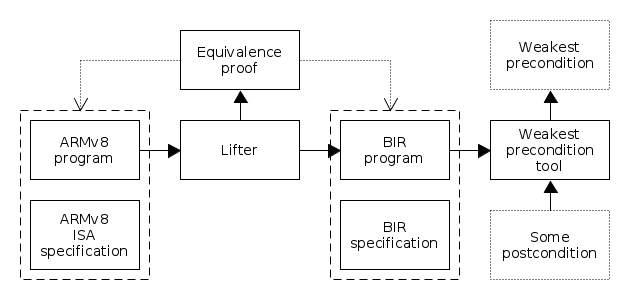
\includegraphics[height=5cm]{figures/holba-overview.png}
	\centering
	\caption{The HolBA framework. The lifter generates a BIR program and an equivalence proof from an ARMv8 program. The equivalence proof establishes a simulation property between the ARMv8 binary program and the generated BIR binary program, showing that they have the same behaviour with respect to the ARMv8 \gls{ISA} specification and the BIR specification. HolBA also support the Cortex-M0 ISA.}
	\label{holba-overview}
\end{figure}

The idea of this work is to translate the formal \gls{NIC} model of \cite{haglund_formal_2016} using \gls{BIR}, then use HolBA's proof-producing weakest precondition tool to prove the same lower-level lemmas than the formal model. With all the lemmas proved, the security properties are implied. Figure \ref{hol-v-bir-nic-model-simple} gives an overview of this idea: using the proof-producing weakest precondition tool to bind together a newly written BIR NIC model and the work done on the formal model.

\section{Intended readers}

In this thesis, formal verification is the central topic. The thesis presents how model a hardware device using a binary analysis platform and presents some formal verification techniques. A reader interested in this topic may find the results presented useful for further work. A casual reader will be presented with a light introduction to the underlying theories and learn some useful ideas for performing software verification. The reader is expected to have a background in Computer Science in general, and knowledge in formal verification will make the thesis easier to digest.

\section{Thesis objective}

The primary goal of this thesis project is to explore verification techniques in order to automate parts, if not all, of the verification process of hardware devices using the HolBA platform. The formal \gls{NIC} model of \cite{haglund_formal_2016} is used as working example.

The ultimate goal would be to obtain a fully automatic pipeline for performing such verifications. However, it is evident that goal isn't reachable in such a small amount of time, or even at all. Thus, this thesis focuses instead on exploring what toolkit is needed in order to facilitate this work.

\section{Delimitations}
\textbf{TODO}: Is that section needed?

\section{Choice of methodology}

This work has been carried out step-by-step toward an ideal goal, i.e. re-establishing all the security properties. On the road, needs have been identified and tools have been implemented in order to tackle them. This approach made sense in this particular work because the needs weren't known in advance, and therefore needed to be identified. This thesis presents the steps taken during this work, the motivations of each tool that have been implemented, and discusses their limitations and future work in the conclusion.


\chapter{Definitions}
\vspace{-1cm}
\textit{This chapter intends to introduce the concepts that are essential to the reader in order to understand the problem that this degree project aims to explore. This includes a presentation of Interactive Theorem Proving and formal proofs in HOL4 and an introduction to \gls{BIR}, completing what has already been said about the \gls{holba} framework in the Introduction.}

\section{Interactive Theorem Proving and HOL4}

Interactive theorem provers are software producing formal proofs, in an
interactive fashion, i.e. a human can step through the proof interactively while the proof assistant provides some automation (like rewriting of terms, arithmetic evaluation, integration with external tools like SMT solvers, \dots). Coq, HOL4 or Isabelle are such tools.

HOL4 \cite{noauthor_hol_nodate} stands for Higher-Order Logic. It is a programming environment deeply embedded into the \gls{SML} programming language enabling to prove theorems and write \gls{proof-producing} programs. Since its first version in 1988, HOL has been focused on hardware verification, and has been successfully used in this domain, as shows its \texttt{examples/} directory \cite{noauthor_canonical_nodate}.

HOL4 is built around a very small kernel: 3 axioms, 10 inference rules, two predefined constants and two types \cite{tuerk_interactive_nodate}\footnote{This is true for the Hol Light Kernel, because the HOL4 kernel has slightly deviated from this simplicity for historical and performance reasons.}. A theorem can only be built using this core, every other higher-level theory must be built from lower-level ones. Furthermore, the kernel is consist of very few lines of code, leaving less space for bugs. Hence, for this reason, the trust needed is far inferior to standard systems.

Several models of different ARM \gls{ISA} have been realized, such as ARMv3, ARMv4, ARMv7 \cite{noauthor_canonical_2019, hutchison_trustworthy_2010} and very recently ARMv8 \cite{armstrong_isa_2019}. These models enable making proofs directly at the ISA level, avoiding the necessity to trust the compiler and enabling to formally verify program behaviours according to the CPU specification. However, this process is tedious and cannot actually be perform by hand. To respond to this problem, \cite{metere_sound_2017} introduced a proof-producing lifter that moves the verification from raw assembly code to an higher-level intermediate representation, and introduced later some supporting tools \cite{lindner_trabin:_2019} in order to automate some of the work. This constitutes the foundation of HolBA.

\section{HolBA's Binary Intermediate Representation (BIR)}

HolBA's Binary Intermediate Representation (BIR) \cite{lindner_trabin:_2019}, introduced in the Introduction, is a machine independent binary representation. It aims to be the simplest possible while still being able to represent all possible binary programs but self-modifying programs. It does so by having a limited syntax---introduced in Table \ref{bir-syntax}---and forbidding implicit side-effects. A statement can only have explicit state changes and can only affect one variable.

\begin{table}[h!]
	\begin{align*}
		prog   & :=~block^{\ast}                                                             \\
		block  & :=~(string~|~integer,~stmt^{\ast},~estmt)                                   \\
		stmt   & :=~\textbf{assign}~(string, exp)~|~\textbf{assert}~(exp)                    \\
        estmt  & :=~\textbf{jmp}~(exp)~|~\textbf{cjmp}~(exp,~exp,~exp)~|~\mathbf{halt}~(exp) \\
		exp    & :=~integer~|~\textbf{var}~string                                            \\
		       & ~~~~|~\textbf{if-then-else}~(exp,~exp,~exp)                                 \\
		       & ~~~~|~\diamond_{u}~exp~|~exp~\diamond_{b}~exp~                              \\
		       & ~~~~|~\textbf{load}~(exp,~exp,~\tau)~|~\textbf{store}~(exp,~exp,~exp,~\tau) 
	\end{align*}
    % exp: string~|~ ??
	\caption{BIR's syntax. Valid BIR programs must be well-typed. $integer$s represent bounded N-bit integers. $\diamond_{u}$ and $\diamond_{b}$ represent respectively unary and binary operators. BIR blocks are tuples, with the first element being its label, the second a list of statements and the third the end statement. BIR syntax contains some other statements that won't be used in this work and that have been omitted. For more information, see \cite{lindner_trabin:_2019}.}
	\label{bir-syntax}
\end{table}

This representation allows to produce proofs more easily that with classical binary representations, whose design are focused on execution speed rather than offline analysis. Moreover, BIR is fully specified and doesn't have unspecified behaviour.

BIR is implemented as a set of HOL4 \textit{datatypes}, and possesses a completely defined semantic. Section \ref{bir-memories-with-smt-solvers} contains a more thorough discussion of the BIR semantic. Section \ref{alice-bob-toy} shows a toy BIR program using the concrete BIR syntax.


\chapter{The BIR NIC model} \label{nic-model}
\vspace{-1cm}
\textit{This chapter intends to discuss about the different ways of implementing an equivalent BIR model from the formal NIC model. It will first offer a brief overview of the formal model. Then, after a discussion about the different possible ways of doing this translation, two approaches will be presented. Finally, the final BIR model will be introduced along with the new tools that have been implemented in order to build it.}


% * Liberté de la méthode et question sur comment traduire le modèle
%
% * Expérimentation en C et avec Alice et Bob (+ CFG (+ interface))
% * Modèle BSL (-> prez de BSL)
%
% * Impossibilité de tout représenter avec BIR (pourquoi?)
%   -> identification (> DepGraph) et fragmentation
%   -> transition vers la preuve

The first step of this work is to 

\section{Overview of the formal NIC model}

The formal NIC model of \cite{haglund_formal_2016} has been designed from reading the hardware specification of the device, because no model nor device driver is freely available.

The NIC model is designed as a transition system with four types of transitions: register read, register write, autonomous, and memory read request reply transitions. They are described by four functions which constitute its public interface: \texttt{read\_nic\_register}, \texttt{write\_nic\_register}, \texttt{nic\_transition\_autonomous} and \texttt{memory\_read\_reply}. Each of these functions update the given initial NIC state, simulating the real behaviour of the NIC. To make the model sound, the state is marked \textit{dead} if the model is asked to describe any transition or operation that is not described by the specification. Dead states represent undefined states and cannot be left with further transitions.

The model is composed of five finite state automata describing the inner transitions of the whole system, each automata describing a part of the NIC. The automata are: initialisation, transmission, transmission teardown, reception and reception teardown. The function \texttt{nic\_execute} performs one autonomous step of one of the five automata. The automaton that takes a step is decided by a scheduler, depending on the NIC inner state. If more that one automata are in a ready state, their order is not deterministic. Each finite state automata is defined as a set of transitions working on NIC states. Each transition takes a NIC state and returns an update one, possibly dead.

Being designed as a transition system, each of the four functions described earlier are loop-free, aspect that is crucial in order to apply contract based verification as described in Section \ref{contract-based-verif}. Each of the transition is implemented as a HOL4 function using exclusively \textbf{if-then-else} and state modification statements. There are no recursive definition. Hence, every function can be seen as some kind of decision tree in which some of the nodes ``mutate'' the state. This idea will be refined later on in Section \ref{visualizing-cfg}.

The five automata are of different complexity, as shown in Table \ref{stats_complexity_formal_nic_model}, with the initialization automaton having only 4 transitions of which only one is autonomous, and the reception automaton being the most complex with 20 transitions. Calling the \texttt{nic\_transition\_autonomous} function makes one of the automata take an autonomous step.

\begin{table}[ht!]
    \centering
    \begin{tabular}{ | l | c | c | c | }
        \hline
        Automaton & \# of (autonomous) transitions & LoC (w/o comments)\\
        \hline
        Initialization & 4 (1) & 21\\
        Transmission & 7 (5) & 182\\
        Transmission teardown & 5 (4) & 67\\
        Reception & 20 (20) & 280\\
        Reception teardown & 7 (6) & 93\\
        \hline
    \end{tabular}
    \caption{Statistics on each of the automata in the formal NIC model.}
    \label{stats_complexity_formal_nic_model}
\end{table}

The NIC state is defined as a nested \textit{datatype}---a record \footnote{Records in HOL4 are analogous to structures in imperative languages.} of records of words, booleans and enumerations. However, there is one exception: the NIC works on a memory data structure, called \texttt{CPPI\_RAM}, which is represented in the formal model as a function from addresses to values.
\todo{explain the problem related to CPPI-RAM?}

The structure of the implementation of \texttt{read\_nic\_register} and \texttt{write\_nic\_register} is similar to the implementation of \texttt{nic\_transition\_autonomous} in terms of the statements they use. \texttt{memory\_read\_reply} is implemented as a non autonomous transition of the transmission automaton.


\section{Translation of the NIC model to HolBA's intermediate language}
% + schema showing multiple ways of implementing the NIC model in BIR

Multiple approaches of translation of the formal NIC model to an equivalent BIR program have been considered:

\begin{itemize}
    \item \textbf{handwritten BIR program}: The most straightforward way would be to directly write the BIR program by hand by looking at the actual formal model and directly converting it to BIR. This is easily feasible because of the limited set of statement used in the implementation of the NIC model which are all representable in the BIR syntax. However, this does not seem optimal if more than one such translation need to be performed. One remedy of this problem would be to implement a set of tools that facilitate the implementation of device models and reduce the boiler plate. This idea is explored in the following Sections \ref{alice-bob-toy} and \ref{impl-real-model}.
    \item \textbf{lifted C program}: An alternative would be to implement the NIC model in a more convenient higher-level programming language, compile it to assembly code and leverage the existing lifter to generate a BIR program. One advantage of this method is the possibility to use existing frameworks and tools that already exist in other languages, in which the ease of development is higher. However, the gained ease of development is maybe not worth the complexity introduced by those steps. The following Section \ref{c-model} experiments this idea.
    \item \textbf{device model specific \gls{IR}}: This idea rejoins the previous one in the sense that it uses an additional intermediate representation (C in the previous idea) to implement the model, then uses some compiler to generate the BIR program (standard C compiler and HolBA's lifter). This idea would have the advantage that it introduces a new higher-level IR that would be common to possible later other device modelisations. Tools could also be developed for this IR. However, this approach would require to develop a new IR and, if we later want to develop a \gls{proof-producing} lifter (compiler) the implementation would be costly, especially since this language would be more complex. The following Section \ref{flowchart-attempt} tries to use visual flowchart language as IR. %This idea has not been explored in this work, where we decided to experiment using existing tools: the lifter, BIR and its supporting tools.
\end{itemize}


\subsection{Using flowcharts as Intermediate Representation} \label{flowchart-attempt}
% essayé flowcharts, simple mais taille grossit très vite, complexe, tedious

As already discussed in the previous Section, the structure of the formal model looks like a tree. Therefore, using flowcharts can be a convenient way to represent such structures. An attempt has been made to design a flowchart representation. Figures \ref{flowchart-scheduler}, \ref{flowchart-tx} and \ref{flowchart-tx_fetch_next_bd} show respectively a preview of the scheduler, transmission automaton and particular transition of this automaton.

\begin{figure}[h]
	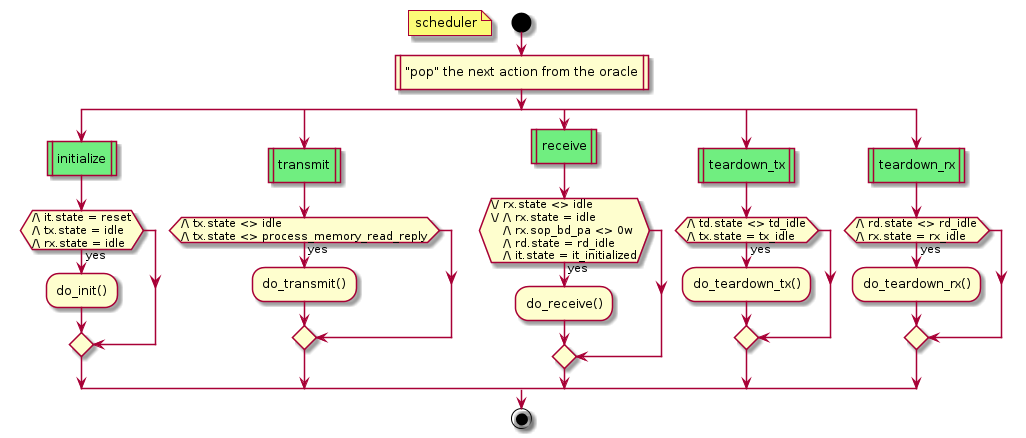
\includegraphics[width=\textwidth]{figures/flowchart-scheduler.png}
	\centering
	\caption{Flowchart of the scheduler of the NIC model. Green nodes represent condition statements, here they represent the value of the popped action from the oracle. The full dot represent the entry point, and the other point the exit point.}
	\label{flowchart-scheduler}
\end{figure}

\begin{figure}[h]
	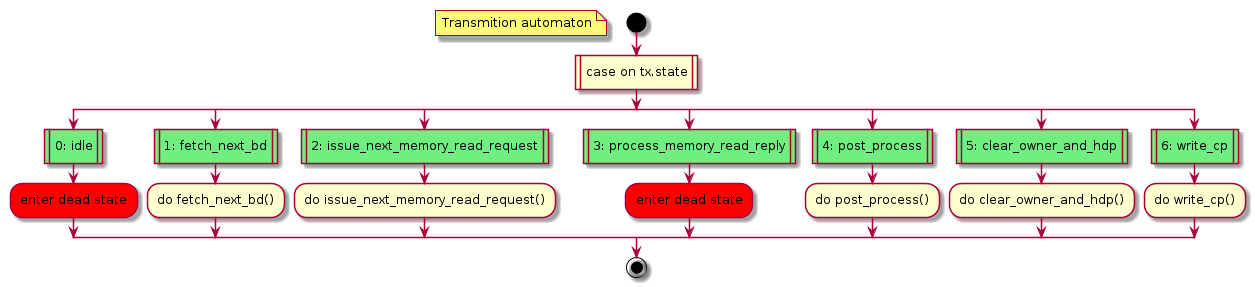
\includegraphics[width=\textwidth]{figures/flowchart-tx.png}
	\centering
	\caption{Flowchart of the transmission automaton of the NIC model. Green nodes are similar to the ones of Figure \ref{flowchart-scheduler}. Red nodes represent non autonomous transitions leading to dead states.}
	\label{flowchart-tx}
\end{figure}

\begin{figure}[h]
	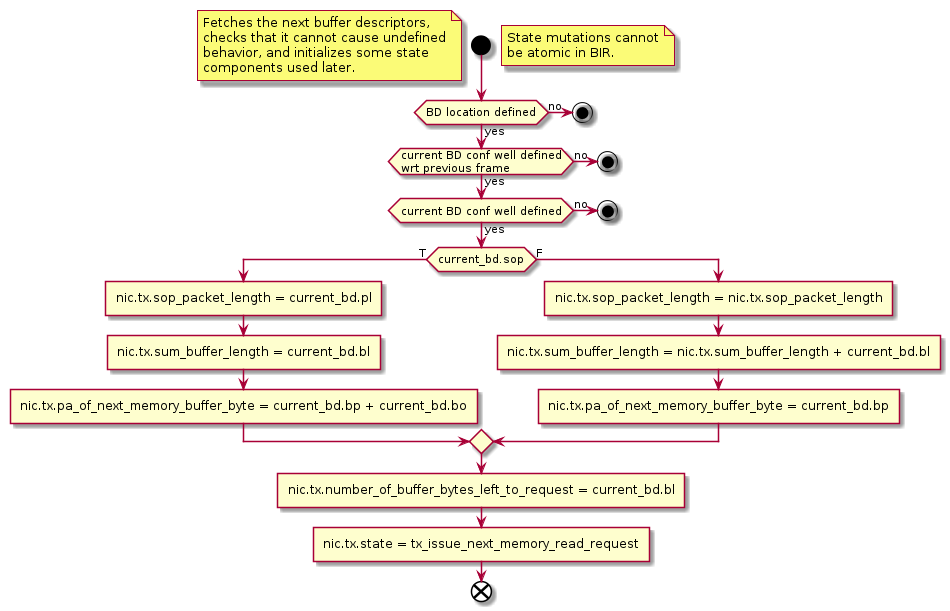
\includegraphics[width=\textwidth]{figures/flowchart-tx_fetch_next_bd.png}
	\centering
	\caption{Flowchart of the \texttt{fetch\_next\_bd} transition of the transmission automaton of the NIC model. The full dot represent the entry point, $\bigotimes$ represents the exit point and the other dots are shorthands to represent dead transitions (the symbols have been changed because of technical limitations of the tool used to draw the diagram).}
	\label{flowchart-tx_fetch_next_bd}
\end{figure}

While this visual representation was useful to get to know the formal NIC model, we encountered several shortcomings:

\begin{itemize}
    \item Flowcharts of each transition rapidly grew in size with the complexity of its formal counterpart. Possible orkarounds include the use of nested diagrams, as it is the case of Figure \ref{flowchart-tx_fetch_next_bd} representing one node of Figure \ref{flowchart-tx}, namely \texttt{fetch\_next\_bd}, or usage of shorter ways of representing common patterns, as it is the case for representing dead transitions on Figure \ref{flowchart-tx_fetch_next_bd}.
    \item It is hard to define a coherent visual language able to represent the full set of features needed in order to realize device models. Additionally, this language must be compatible or easily translatable to BIR.
    \item It is hard to design a textual representation of this visual language other than conventional programming languages, so using such representation would require a consequent implementation effort in order to implement all the tools needed to use it.
\end{itemize}

For those reasons, it has been decided to not go further with this visual representation, and to focus instead of existing tools of the HolBA platform.

\subsection{Writing the model in C} \label{c-model}
% Problem: we don't want to reason with the stack

One-to-one translation of the transmission automaton, scheduler, state and \textit{CPPI\_RAM} related definitions of the formal model has been realized in C. This translation has been quite easy to perform and has been completed in around four hours. No difficulty arisen during this translation. Regarding the NIC state, C has all types needed to represent it. An array has been used to represent the function type of \textit{CPPI\_RAM}. Enumerations have been used in order to represent HOL4 enumerations. While not optimal is conventional usage of C because of their non restricted usage allowed by the C language (they can be freely modified as integers without checking their validity in C, while HOL4 and functional languages in general are restrictive and force to use correct values), enumerations are enough if used correctly and aware of those shortcomings. However, when studying the compiled assembly code and lifted BIR program, we noticed that all the convenient naming that we can use in the formal or the C model is lost and replaced with abundant usage of the stack. While this is completely normal behaviour for a C compiler, this is not convenient when performing later proofs on the model: we would first need to rename them in the proof using some definitions, and this process would be lengthy and cumbersome (if not automated), resulting in more code than if the model had been directly written in BIR in the first place. This experiment made us realize that writing the model is a rapid operation and that we should rather focus on making the verification step as smooth as possible, because it is the most difficult to carry out.

For those reasons, it has been decided to try using BIR directly to write the NIC model. First, Section \ref{alice-bob-toy} presents a first prototype that has been realized in order to visualize the shape of a BIR program representing the NIC model, and identify the tools that would be needed in order to reduce the boilerplate of such implementation in BIR.


\subsection{A story of Alice and Bob} \label{alice-bob-toy}
% BIR toy model



\subsection{Visualizing the CFG} \label{visualizing-cfg}


\subsection{BSL: BIR Simple Language} \label{bsl}

\subsection{Device model specific BIR helpers}

\subsection{Implementing the real model} \label{impl-real-model}
% model not-complete model (focus on key parts)


\section{Overview of the formal proof on the NIC model}

\subsection{BIR limitations}
\subsection{DepGraph}



% [Proving properties]
%
% * Introduction des WP
%   - Rappels sur le WP existant dans HolBA
% * Explication de l'utilisation de SMT solver
%   - Ajout des arrays dans l'export existant
%   - Experiments with SMT (before and after array): without and with BIR
%   --- With BIR needed BIR EXP -> Words (why?)
%   ----- Non proof-producing + explain why (mention that PP has been done in the proof)
% * Non proof-producing WP lib
%   + easy
%   - proof-producing would have been feasible
%     -> but would have took more time, that's not the aim of the thesis
% * BIR PP because huge WP BIR expressions
% * WP tests
%   - simple
%   - Gauss analysis (how to handle loop, mult problem with SMT)
%   - memories
%   - cjmp bug?
%   - explain the simp (ie. the subst theory) + the exponential growth issue ? should I explain it ?
% * Using the WP tool on simple properties on the BIR NIC model
%   - Remind about the impossibility to express certain properties using contracts
% * Explain the PP proof
%   - Whiteboard explanation
%   - Pen and paper proof
%   - About implementation
%   --- About PP BIR to words

\chapter{Contract based verification} \label{contract-based-verif}
\vspace{-1cm}
\textit{This chapter will discuss about experiments carried out in order to perform formal verification on the \gls{NIC} model written in \gls{BIR}. It will first introduce contract based verification, its current status in the \gls{holba} platform, and the non \gls{proof-producing} contract based library that has been implemented in this work. It will then present some contract based verifications that has been performed in a non proof-producing fashion on example programs and on the NIC model of the previous section.}

\section{Hoare triples}

Contract based verification is a powerful approach for verifying programs. For a given program $prog$ consisting of a list of instructions and two predicates $P$ and $Q$ called respectively pre- and postcondition, a Hoare triple \htriple{P}{prog}{Q} states that when executing the program $prog$ from a state $S$ terminates in a state $S'$, if $P$ holds in $S$ then $Q$ will hold in $S'$ (Equation \ref{ht_def}). Hereafter, we assume programs and states to be well-typed.

\begin{equation}
  \htriple{P}{prog}{Q} \triangleq S' = exec(S, prog) \implies P(S) \implies Q(S')
  \label{ht_def}
\end{equation}

For example, \htriple{P}{\varnothing}{P} holds because an empty program doesn't change the state of the execution. \htriple{n=1}{n:=n+1}{even(n)}, with $n \in \mathbb{N}$, holds because $1+1=2$, which is even.

In order to perform the verification, the Hoare logic introduces a set of axioms describing the effect of each instruction of a given language over the execution state \cite{hoare_axiomatic_1969}. For an assignment $x:=f$ where $x$ is a variable identifier and $f$ an expression without side-effects, Equation \ref{axiom_assignment_def} defines the axiom of assignment, where $P[f/x]$ denotes the substitution of all occurrences of $x$ by $f$ in $P$.

\begin{equation}
  \htriple{P[f/x]}{x:=f}{P}
  \label{axiom_assignment_def}
\end{equation}

\todo{Introduce labels? \htriple{l1:P}{l1->\{l2,l3\}}{l2:Q,l3:Q'}}

\section{Weakest precondition derivation}

While Hoare logic introduces sufficient preconditions, Dijkstra introduced the concept of necessary and sufficient preconditions, called ``weakest'' preconditions. Such weakest preconditions can be automatically derived from a program $prog$ and a postcondition $Q$. Let's call $\WP(prog, Q)$ such a weakest precondition. Then, from Equation \ref{ht_def} follows:

\begin{equation}
  \forall (prog, Q),
  \htriple{\WP(prog,Q)}{prog}{Q}
  \label{ht_wp_eq}
\end{equation}

For the program $n:=n+1$ mentioned above, we can generate the weakest precondition for the postcondition $even(n)$. First, we can rewrite $even(n)$ as $n~MOD~2 = 0$ with $MOD$ denoting the arithmetic modulo. Then, we derive the weakest precondition of the statement $n:=n+1$ by transforming the predicate $n~MOD~2 = 0$ by substituting all occurrences of $n$ by $n+1$:

\begin{equation}
  \WP(``n:=n+1'',n~MOD~2 = 0)=(n+1~MOD~2 = 0)
  \label{wp_comp_n_inc_even}
\end{equation}

From the properties of the modulo, we can simplify $n+1~MOD~2 = 0$ to $n~MOD~2 = 1$ or $odd(n)$. Therefore, \htriple{odd(n)}{n:=n+1}{even(n)}, i.e. incrementing the value of an odd integer variable by one makes it even.

While the triple \htriple{n=1}{n:=n+1}{even(n)} uses a sufficient precondition for establishing its postcondition, the triple \htriple{odd(n)}{n:=n+1}{even(n)} uses the weakest precondition. The later being the weakest precondition of the former, the two contracts are in relation:

\begin{equation}
  n=1 \implies odd(n)
\end{equation}

More generally, for a triple \htriple{P}{prog}{Q} to hold, $P$ must be stronger than the weakest precondition, i.e. we need to prove that $P \implies \WP(prog, Q)$.

\todo{Here and above, should we mention/explain termination?}

\begin{equation}
  (P \implies \WP(prog, Q)) \implies \htriple{P}{prog}{Q}
  \label{p_imp_wp}
\end{equation}

\section{Using SMT solvers to prove contracts} \label{using-smt-to-prove-contracts}

From Equation \ref{p_imp_wp} we see that, in order to prove that a triple \htriple{P}{prog}{Q}, we need to prove $P \implies \WP(prog, Q)$. While multiple methods exist to perform such proofs, \acrshort{SMT} solvers offer a convenient and automatic solution.

\acrfull{SMT} problem is a decision problem for logical formulas with respect to combinations of background theories such as arithmetic, bit-vectors, arrays, and uninterpreted functions \cite{nikolaj_bjorner_programming_2019}. \gls{SMT} problem is a generalization of \gls{SAT} problem supporting more theories. When given a formula, a \gls{SMT} solver decides if the formula is satisfiable, i.e. if there exist a valuation of its variables where the formula evaluates to true. As a \gls{SMT} solver can fail to decide a given instance, there are three possible outputs: ``satisfiable'', ``unsatisfiable'' and ``unknown''. Another useful feature of some \gls{SMT} solvers is the ability to ask for a satisfying model, which represents a counter-example of a false predicate.

A predicate $P$ holds if it evaluates to true for all possible values of its variables \todo{isn't that the definition of tautologies?}. Alternatively, the negation of a predicate $\neg P$ holds if there exist no valuation of its variables where the predicate evaluates to true, i.e. if the instance is unsatisfiable. Therefore, if a \gls{SMT} solver report that $\neg P$ is ``unsatisfiable'', then $P$ holds.

Another way of thinking about how to prove logical formulas with \gls{SMT} solvers is by using De Morgan's Laws: we know that $\neg (P \implies \WP) \equiv (P \land \neg \WP)$. Therefore, proving that $\neg (P \implies \WP)$ is ``unsatisfiable'' using an \gls{SMT} solver can be seen as proving that there exist no model where $P$ holds and $\WP$ doesn't.

\subsection{Getting started with the BitVector theory}

To reason about fixed-size integers, \gls{SMT} solvers often implement a ``BitVector'', or ``FixedSizeBitVectors'', theory. In order to understand its particularities, we can try to prove Equation \ref{bv_eq1}. Hereafter, we will use Z3, a popular and efficient \gls{SMT} solver implemented by Microsoft Research\footnote{Z3 is available on GitHub at \url{https://github.com/Z3Prover/z3/}.}, and SMT-LIB 2.0, which is a standard format for \gls{SMT} solvers \cite{barrett_satisfiability_2016}. Listing \ref{bv_eq1_smtlib} shows the SMT-LIB 2.0 representation of this proof attempt.

\begin{equation}
    \forall x.~ x + 1 > x, \text{with $x$ an unsigned 32-bit integer}
    \label{bv_eq1}
\end{equation}

\begin{lstlisting}[
    language=Lisp,
    backgroundcolor=\color{codebackcolour},
    commentstyle=\color{codegreen},
    keywordstyle=\color{magenta},
    stringstyle=\color{codepurple},
    label=bv_eq1_smtlib,caption=SMT-LIB 2.0 representation of Equation \ref{bv_eq1}.,
    frame=tb,basicstyle=\footnotesize\ttfamily]
(declare-const x (_ BitVec 32))
(assert (not
  (bvugt (bvadd x (_ bv1 32)) x)))
(check-sat)
(get-model)
\end{lstlisting}

When given Listing \ref{bv_eq1} as input, Z3 gives the following output:

\begin{lstlisting}[
    language=Lisp,
    backgroundcolor=\color{codebackcolour},
    commentstyle=\color{codegreen},
    keywordstyle=\color{magenta},
    stringstyle=\color{codepurple},
    label=bv_eq1_output,caption=Z3 output for Listing \ref{bv_eq1_smtlib}.,
    frame=tb,basicstyle=\footnotesize\ttfamily]
sat
(model (define-fun x () (_ BitVec 32) #xffffffff))
\end{lstlisting}

Z3 is telling us that Equation \ref{bv_eq1} is false, and gives a counterexample: $x=2^{32}-1$. Indeed, with this value of $x$, $x+1$ wraps around and result in $0$ which is smaller that $2^{32}-1$. This behaviour is due to the bounded nature of fixed-size integers. The correct equation here would be:

\begin{equation}
    \forall x.~ x \neq 2^{32}-1 \implies x+1>x, \text{with $x$ an unsigned 32-bit integer}
    \label{bv_eq2}
\end{equation}

Listing \ref{bv_eq2_smtlib} and \ref{bv_eq2_output} show the input and output of Z3 used to successfully prove Equation \ref{bv_eq2}.

\begin{lstlisting}[
    language=Lisp,
    backgroundcolor=\color{codebackcolour},
    commentstyle=\color{codegreen},
    keywordstyle=\color{magenta},
    stringstyle=\color{codepurple},
    label=bv_eq2_smtlib,caption=SMT-LIB 2.0 representation of Equation \ref{bv_eq2}.,
    frame=tb,basicstyle=\footnotesize\ttfamily]
(declare-const x (_ BitVec 32))
(assert (not
  (bvugt (bvadd x (_ bv1 32)) x)))
(assert (not (= x #xffffffff)))
(check-sat)
\end{lstlisting}

\begin{lstlisting}[
    language=Lisp,
    backgroundcolor=\color{codebackcolour},
    commentstyle=\color{codegreen},
    keywordstyle=\color{magenta},
    stringstyle=\color{codepurple},
    label=bv_eq2_output,caption=Z3 output for Listing \ref{bv_eq2_smtlib}.,
    frame=tb,basicstyle=\footnotesize\ttfamily]
unsat
\end{lstlisting}

\section{Contract based verification in HolBA} \label{contract-verif-holba}

\gls{holba} provides a \gls{proof-producing} tool for automatically deriving weakest preconditions on loop-free \gls{BIR} programs whose control flow can be statically identified \cite{lindner_trabin:_2019}. This tool is proof-producing in that it proves Theorem \ref{triple_wp_thm} which is the instantiation of Definition \ref{holba_wp_ht_thm}, with $(p,~entry\_l,~end\_ls)$ defining the program, $wp$ the derived weakest precondition, $post$ the given postcondition.

\begin{equation}
    bir\_exec\_to\_labels\_triple~prog~entry\_l~end\_ls~\mathbf{wp}~post
    \label{triple_wp_thm}
\end{equation}

\begin{small}
\begin{equation}
\begin{split}
    \vdash \forall &(prog :\alpha~bir\_program\_t)~(entry\_l :bir\_label\_t)%
    ~(end\_ls :bir\_label\_t \rightarrow bool)\\
    & (pre :bir\_exp\_t)~(post :bir\_exp\_t).\\
    & bir\_exec\_to\_labels\_triple~prog~entry\_l~end\_ls~pre~post \Leftrightarrow\\
    & ~~\forall~(s~:bir\_state\_t)~(r~:\alpha~bir\_execution\_result\_t).\\
    & ~~~~~~~~~~~~~~~~~bir\_env\_vars\_are\_initialised~s.bst\_environ~(bir\_vars\_of\_program~prog)\\
    & ~~~~~~\implies s.bst\_pc.bpc\_index~=~0~\land~s.bst\_pc.bpc\_label~=~entry\_l\\
    & ~~~~~~\implies s.bst\_status~=~BST\_Running\\
    & ~~~~~~\implies bir\_is\_bool\_exp\_env~s.bst\_environ~pre\\
    & ~~~~~~\implies bir\_eval\_exp~pre~s.bst\_environ~=~bir\_val\_true\\
    & ~~~~~~\implies bir\_exec\_to\_labels~end\_ls~prog~s~=~r\\
    & ~~~~~~\implies \exists~(obs~:\alpha~list)~(step\_count~:num)%
    ~(pc\_count~:num)~(s'~:bir\_state\_t).\\
    & ~~~~~~~~~~~~~~~~~~~~~~~~r~=~BER\_Ended~obs~step\_count~pc\_count~s'\\
    & ~~~~~~~~~~~~~~~~~~~\land~s'.bst\_status~=~BST\_Running\\
    & ~~~~~~~~~~~~~~~~~~~\land~bir\_is\_bool\_exp\_env~s'.bst\_environ~post\\
    & ~~~~~~~~~~~~~~~~~~~\land~bir\_eval\_exp~post~s'.bst\_environ~=~bir\_val\_true\\
    & ~~~~~~~~~~~~~~~~~~~\land~s'.bst\_pc.bpc\_index~=~0~\land~s'.bst\_pc.bpc\_label~\in~end\_ls
\end{split}
\label{holba_wp_ht_thm}
\end{equation}
\end{small}

It is to be noted that this tool doesn't produce a theorem stating that the generated expression is actually \textit{the} weakest precondition. However, this theorem isn't needed to perform contract-based verification if the generated ``weakest'' precondition is weak enough so that our precondition can imply it. However, without this theorem it is impossible to prove that a given precondition $P$ isn't strong enough to establish the postcondition. We will still use the term ``weakest precondition'' as it is in practice how we are using this tool.

Definitions \ref{holba_wp_ht_thm} introduces additional conditions about well-typedness and initialization that are needed in BIR today\footnotemark, as well as the notion of ``Block Program Counter'' for multi-statement blocks. %However, those can easily be proved and we are then left with the Hoare triple definition expressed in terms of evaluating the pre- and post-conditions in the initial and final state.

\footnotetext{Removal of the need of initialization is being discussed at the time of the writing, because actual hardware registers and memories are in facts always initialized: \url{https://github.com/kth-step/HolBA/issues/63}}

This tool doesn't provide a simple interface to compute weakest preconditions for a given program and postcondition, nor does it provide and support for proving the relation between the precondition and the weakest precondition. Then, in order to prove that the Hoare triple holds from this generated Theorem \ref{triple_wp_thm}, we need to prove:

\begin{equation} 
    bir\_exec\_to\_labels\_triple~p~entry\_l~end\_ls~\mathbf{pre}~post
    \label{triple_pre_thm}
\end{equation}

Assuming well-typedness and initialization, after rewriting the definition of $bir\_exec\_to\_labels\_triple$, we have to show $bir\_eval\_exp~\mathbf{wp}~s.bst\_environ~=~bir\_val\_true$ in order to prove our goal using the \textit{modus ponens} with Theorem \ref{triple_wp_thm}. This correspond to proving the following implication:

\begin{small}
    \begin{equation}
        \begin{split}
            &bir\_eval\_exp~\mathbf{pre}~s.bst\_environ~=~bir\_val\_true\\
            &\implies bir\_eval\_exp~\mathbf{wp}~s.bst\_environ~=~bir\_val\_true
        \end{split}
        \label{eval_pre_imp_eval_wp}
    \end{equation}
\end{small}

In Equation \ref{eval_pre_imp_eval_wp} we can recognize Equation \ref{p_imp_wp} that we discussed how to prove using \gls{SMT} solvers in Section \ref{using-smt-to-prove-contracts}. However, the expressions are expressed as BIR expressions. We then have to find a way to use an SMT solver. This is the focus of the following of this thesis. Section \ref{impl-non-pp-wp-lib} will use a non \gls{proof-producing} method for translating those BIR expressions into an equivalent formula that SMT solvers can work on, then focus on automating the whole verification process. Chapter \ref{trustful-nic-analysis} will complete this proof and use it to lift properties that have been proved on the BIR implementation to the \gls{NIC} model. The following Section \ref{bir-memories-with-smt-solvers} will discuss how to make proofs about BIR memories using \gls{SMT} solvers.

\section{BIR memories and SMT solvers} \label{bir-memories-with-smt-solvers}

% Mention SMT-LIB logics?
% Mention proof reconstruction?

HOL4 features a library for interfacing \gls{SMT} solvers and HOL4, called \textit{HolSmtLib}. This library supports Yices 1 and Z3 as external provers. Yices 1 being an abandoned project that doesn't support SMT-LIB 2.0, we will focus on Z3 and the standard format SMT-LIB 2.0 \cite{barrett_satisfiability_2016}. While \textit{HolSmtLib} supports export for some SMT-LIB 2.0 theories, it doesn't support the \textit{ArraysEx} theory and doesn't know about BIR. In Section \ref{contract-verif-holba}, we discussed the translation from BIR expressions to \textit{wordsTheory}. However, this theory doesn't contain anything about memories or arrays in general. Therefore, some modifications are needed.

BIR memories are semantically defined as functions from addresses to values. 

There exist five types of BIR expressions operating directly on memories (cf. Listing \ref{bir_bin_exp_def} for the list of BIR expressions, and Section \ref{exporting-bir-to-smt} for a more precise discussion of the BIR semantic):

\begin{itemize}
    \item \texttt{BExp\_Den}: this operation enables reading values from the environment. It is analogous to reading registers or the memory in assembly programs. This operation semantically equivalent to free variables that \textit{HolSmtLib} already support.
    \item \texttt{BExp\_MemEq}: this operation is the equality binary operation on BIR memories. This operation is semantically equivalent to equality between its operands. \textit{HolSmtLib} already supports this operation.
    \item \texttt{BExp\_Store}: this operation is used to represent memory writes. It is semantically defined as successive function updates of consecutive segments of the word being stored, because the length of the memory value-type can be less or equal than the length of values stored in the memory. A function update in \textit{combinTheory} is defined with Definition \ref{combin_UPDATE_def}. \textit{HolSmtLib} cannot currently export function update operations.
    \item \texttt{BExp\_Load}: this operation is used to read from memories. BIR memories are semantically defined as functions from addresses to values. A function application in \textit{combinTheory} is defined with Definition \ref{combin_APP_def}. Then, a memory load operation is the concatenation of multiple function application of consecutive addresses. \textit{HolSmtLib} supports function application of uninterpreted functions only.
\end{itemize}

\begin{equation}
    \vdash \forall a~b.~a~\text{=+}~b = (\lambda f~c.~\text{if}~a = c~\text{then}~b~\text{else}~f~c)
    \label{combin_UPDATE_def}
\end{equation}

\begin{equation}
    \vdash \forall x~f.~x~\text{:>}~f = f~x
    \label{combin_APP_def}
\end{equation}

We saw in the previous list that we need to implement the support for \textit{combinTheory} function update and application in the \textit{HolSmtLib} SMT-LIB 2.0 exporter. Since we only need two operations on the memory, load and store, the \textit{ArraysEx} theory is a good fit.

SMT-LIB 2.0 \cite{smtlib} defines the \textit{ArraysEx} theory using the three following axioms:

\begin{lstlisting}[
    language=Lisp,
    backgroundcolor=\color{codebackcolour},
    commentstyle=\color{codegreen},
    keywordstyle=\color{magenta},
    stringstyle=\color{codepurple},
    label=smtlib_arrayex_axioms,caption=SMT-LIB 2.0 axioms of the \textit{ArrayEx} theory.,
    frame=tb,basicstyle=\footnotesize\ttfamily]
(forall ((a (Array s1 s2)) (i s1) (e s2))
  (= (select (store a i e) i) e)) 

(forall ((a (Array s1 s2)) (i s1) (j s1) (e s2))
  (=> (distinct i j)
      (= (select (store a i e) j) (select a j))))

(forall ((a (Array s1 s2)) (b (Array s1 s2)))
  (=> (forall ((i s1)) (= (select a i) (select b i)))
      (= a b)))
\end{lstlisting}

If those axioms hold in \textit{combinTheory} then the translation is sound. \textit{combinTheory}'s \textit{UPDATE\_APPLY} theorem in Equation \ref{combin_UPDATE_APPLY} is equivalent to the first two theorems, the first and the second conjunct corresponding respectively to the first and the second axiom. The third axiom can be proved using both \textit{combinTheory}'s \textit{APP\_def} theorem (Theorem \ref{combin_APP_def}) and \textit{boolTheory}'s \textit{EQ\_EXT} theorem (Theorem \ref{bool_EQ_EXT})

\begin{equation}
    \begin{split}
        \vdash &  ~~~~ \forall a~x~f.~(a~\text{=+}~x)~f~a = x\\
               & \land \forall a~b~x~f.~a \neq b \implies ((a~\text{=+}~x)~f~b = f~b)
    \end{split}
    \label{combin_UPDATE_APPLY}
\end{equation}

\begin{equation}
    \vdash \forall f~g.~(\forall x.~f~x = g~x) \implies (f = g)
    \label{bool_EQ_EXT}
\end{equation}

Since this translation is sound, it has been added in \textit{HolSmtLib}. The translation is direct: from \texttt{:>} and \texttt{=+} to respectively \texttt{select} and \texttt{store}. Section \ref{addreq_test} presents a test using BIR memories.



\chapter{Implementation of a non proof-producing automatic contract verification library} \label{impl-non-pp-wp-lib}
\vspace{-1cm}
\textit{In the previous section, we learned about contract verification and the current status of \gls{holba}'s implementation. To perform verification on the \gls{NIC} model, we would like to automate the process as much as possible. \gls{holba} currently offers tools for automatic weakest precondition generation, therefore we need to close the gap between BIR expression and SMT solvers, as well as to implement a convenient interface on top.}

\section{Exporting BIR expressions to SMT solvers} \label{exporting-bir-to-smt}

As an intermediate language for formal verification, \gls{BIR} possesses a precise semantic. The semantic of BIR expressions is expressed as a set of definitions \todo{axioms?} describing what are the equivalent operations using \textit{wordsTheory} and \textit{combinTheory}. These theories contains definitions and theorems about ``words'', i.e. bounded $N$-bit integers that are used to reason about integer types in programming languages and hardware memory in general, and function application and update used for BIR memories as already discussed in Section \ref{bir-memories-with-smt-solvers}. For example, the semantic of binary operators in BIR is defined with the following theorems\footnotemark:

\footnotetext{Theorems \ref{bir_bin_exp_GET_OPER_def} and \ref{bir_bin_exp_def} have been reduced to only two operators and well-typed 64-bit expressions.}

\begin{small}
    \begin{equation}
        \begin{split}
            \vdash~&bir\_bin\_exp\_GET\_OPER~BIExp\_And = words\_and\\
                   &\land bir\_bin\_exp\_GET\_OPER~BIExp\_Or = words\_or\\
        \end{split}
        \label{bir_bin_exp_GET_OPER_def}
    \end{equation}
    \begin{equation}
        \begin{split}
            \vdash~&\forall (bin\_op :bir\_bin\_exp\_t)~(w1 :word64)~(w2 :word64).\\
                   &~~~~~bir\_bin\_exp~bin\_op~(Imm64~w1)~(Imm64~w2)\\
                   &~~~~~= Imm64~(bir\_bin\_exp\_GET\_OPER~bin\_op~w1~w2)
        \end{split}
        \label{bir_bin_exp_def}
    \end{equation}
\end{small}

Similarly, a set of definitions and theorems describe the semantic of operations on BIR memories. However, correct handling of endianness, alignment and genericity over the size of memories cells and addresses, these definitions and theorems are pretty complicated to work with. The same is true for the semantic of operations on BIR variables, because of well-typedness and initialization.

For this reason---i.e. writing \gls{proof-producing} code is costly---, I decided to write a non-proof producing function \texttt{bir\_exp\_to\_words} that translates BIR expressions to the equivalent words expression. The obvious downside of such a function is that we now have to trust the translation to be sound, because we no longer get any guarantee from the theorem prover. However, development time is dramatically decreased and offers more time for experimenting. Moreover, this function can later be implemented in a proof-producing way for more trustful verification. Then, in order to have a high confidence of correctness, software engineering practices apply:

\begin{itemize}
    \item write small and understandable pieces of code and compose them, and
    \item write a comprehensive suite of tests.
\end{itemize}

BIR expressions are defined as a HOL4 algebraic data type in Listing \ref{bir_exp_t_def}. Hence, in order to translate BIR expressions to words expressions, we need to handle every variant. This has been done \footnote{Code available here: \url{https://github.com/kth-step/HolBA/commit/2fcca54dcb04a20716e7697f64b5a4578f8a8af9}} using an exhaustive \texttt{if-then-else} statement\footnotemark. The code is mostly destructuring HOL4 terms and creating new \textit{wordsTheory} and \textit{combinTheory} terms. In order to obtain an easily reviewable code, a balance between expressivity and conciseness has to be carefully decided. Table \ref{bir_exp_to_words_variants_loc} shows that the length of each variant is relatively small in terms of lines of codes, from 1 line for constants to 51 for memory store expressions. This achieves the first point of the previous list.

\footnotetext{Pattern matching would have been optimal, but isn't possible because of how HOL4 is embedded in SML.}

Testing of \texttt{bir\_exp\_to\_words} has been done using a set of $(bir\_exp,expected)$ couples with increasing complexity, where \texttt{bir\_exp\_to\_words} is used to translate each $bir\_exp$ and the result is compared to $expected$. Then, BIR expression being defined as an algebraic data type, nesting of BIR expressions follow naturally. This achieves the second point of the previous list.

\begin{lstlisting}[
    label=bir_exp_t_def,caption=bir\_exp\_t definition.,
    frame=tb,basicstyle=\footnotesize\ttfamily]
Datatype `bir_exp_t =
    BExp_Const      bir_imm_t
  | BExp_Den        bir_var_t

  | BExp_Cast       bir_cast_t bir_exp_t bir_immtype_t

  | BExp_UnaryExp   bir_unary_exp_t bir_exp_t
  | BExp_BinExp     bir_bin_exp_t bir_exp_t bir_exp_t
  | BExp_BinPred    bir_bin_pred_t bir_exp_t bir_exp_t
  | BExp_MemEq      bir_exp_t bir_exp_t

  | BExp_IfThenElse bir_exp_t bir_exp_t bir_exp_t

  | BExp_Load       bir_exp_t bir_exp_t bir_endian_t bir_immtype_t
  | BExp_Store      bir_exp_t bir_exp_t bir_endian_t bir_exp_t`
\end{lstlisting}

\begin{table}[ht!]
    \centering
    \begin{tabular}{ | l | c | }
        \hline
        \texttt{bir\_exp\_t} variant & Lines of code\\
        \hline
        BExp\_Const & 1\\
        BExp\_Den & 21\\
        BExp\_Cast & not implemented\\
        BExp\_UnaryExp & 8\\
        BExp\_BinExp & 9\\
        BExp\_BinPred & 10\\
        BExp\_MemEq & 10\\
        BExp\_IfThenElse & 9\\
        BExp\_Load & 48\\
        BExp\_Store & 51\\
        \hline
    \end{tabular}
    \caption{Length of each \texttt{bir\_exp\_t} variant in the implementation of \texttt{bir\_exp\_to\_words}.}
    \label{bir_exp_to_words_variants_loc}
\end{table}

\section{Pretty-printing to visualize huge BIR expressions}

When working with complex constructs, the need of visualization techniques often arise. Generated weakest preconditions grow quickly with the number of statements in a program, linearly or exponentially depending on the type of statements---control flow statements produce exponential growth. While clever techniques can be implemented to keep their size reasonable \cite{lindner_trabin:_2019}, we often need to read and analyze them.

Printing of BIR terms in general is very verbose. For example, the expression \ref{pp_ex_math_exp} with a 64-bit $x$ integer defined using the BSL code in Listing \ref{pp_ex_bsl_code} yields the printing in Figure \ref{pp_ex_default_printing} using HOL4's default printing capabilities.

\begin{equation}
    \text{if}~~(x \leq 100) \lor (y + 1 > 10) \lor (x + y \leq 20)~~\text{then}~~2 \times x~~\text{else}~~3 \times y + 1
    \label{pp_ex_math_exp}
\end{equation}

\begin{lstlisting}[
    language=Caml,
    backgroundcolor=\color{codebackcolour},
    commentstyle=\color{codegreen},
    keywordstyle=\color{magenta},
    stringstyle=\color{codepurple},
    label=pp_ex_bsl_code,caption=BSL code,
    frame=tb,basicstyle=\footnotesize\ttfamily,
    float,floatplacement=H]
bite (
  borl [
    ble ((bden o bvarimm64) "x", bconst64 100),
    bnot (ble (bplus ((bden o bvarimm64) "y",
                      bconst64 1),
               bconst64 10)),
    ble (bplus ((bden o bvarimm64) "x",
                (bden o bvarimm64) "y"),
         bconst64 20)
  ],
  bmult ((bden o bvarimm64) "x", bconst64 2),
  bplus (bmult ((bden o bvarimm64) "x", bconst64 3),
         bconst64 1))
\end{lstlisting}

\begin{figure}[!h]
	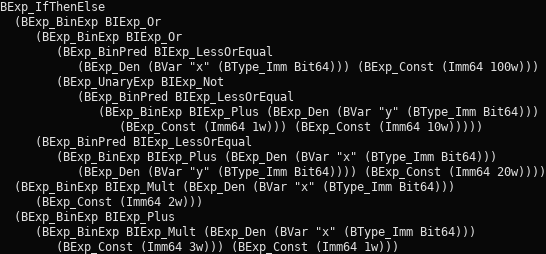
\includegraphics[width=\textwidth]{figures/pp_ex_default_printing.png}
	\centering
	\caption{Default HOL4 printing}
	\label{pp_ex_default_printing}
\end{figure}

This expression is relatively small and yet the printed term is 17 lines long. Compared to the BSL expression that is 8 lines long\footnotemark, that is a two time increase in size. Moreover, lines are long and verbose: for example, a ``less-than'' binary expression is written as ``\texttt{BExp\_BinPred BIExp\_LessOrEqual e1 e2}''. Comparatively, the math expression ``$e1 \leq e2$'' and BSL expression ``\texttt{ble e1 e2}'' are shorter and arguably more readable.

\footnotetext{8 lines correspond to the length in documents where line length is limited to 100 characters, instead of the 60 in the report.}

To answer to these kinds of issues, HOL4 provides the ability to implement ``pretty-printers'', which are custom printing functions for a given type. Four pretty-printers have been implemented to shorten the verbosity of the printed representation and to add colors to the output. Figure \ref{pp_ex_pretty_printing} shows the same expression printed with the pretty-printers enabled.

\begin{figure}[!h]
	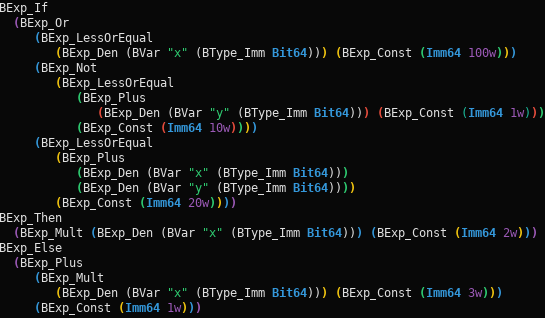
\includegraphics[width=\textwidth]{figures/pp_ex_pretty_printing.png}
	\centering
	\caption{Same expression printed with the pretty-printer enabled}
	\label{pp_ex_pretty_printing}
\end{figure}

The pretty-printers introduce a set of features:

\begin{itemize}
    \item Simplification of verbose constructs as discussed before (e.g. \texttt{BExp\_BinExp BIExp\_Or} is written as \texttt{BExp\_Or}).
    \item Different representation of ``if-then-else'' statements, simplifying reading the expression when either the condition or the ``then'' expression are very long.
    \item Consistent breaking---new lines---of long expressions, because the default printer isn't aware of the structure of printed expressions. In Figure \ref{pp_ex_default_printing}, we can see inconsistent breaking in addition and multiplication binary operations.
    \item Highlighting of types, facilitating debugging when the expression isn't well-typed.
    \item Highlighting of all strings, facilitating reading labels and variable names.
    \item Gathering of nested binary expressions of the same type on the same level. We can see this feature in Figure \ref{pp_ex_pretty_printing} with the two nested ``or'' binary operators, where the three operands are printed on the same level.
    \item Rainbow parenthesis, i.e. matching pairs of parenthesis are printed in the same color. This feature is really useful when reading long expression in order to quickly identify where a sub-expression ends.
\end{itemize}

\section{Implementing a convenient interface} \label{impl_convenient_ht_interface}

In order to perform a high number of proofs on the \gls{NIC} model, we want to hide as much as possible the implementation details of the contract verification procedure. Ideally, we want a function ``\texttt{prove\_contract}'' taking a program fragment, a pre- and a post-condition as parameters, and producing a proof about the Hoare triple if the contract holds or a comprehensive and useful error message if it doesn't. Listing \ref{ideal_interface_prove_contract} shows the ideal interface that we would want, and Listing \ref{interface_prove_contract} shows the actual interface that have been implemented.

\begin{lstlisting}[
    language=Caml,
    backgroundcolor=\color{codebackcolour},
    keywordstyle=\color{magenta},
    label=ideal_interface_prove_contract,caption=Ideal interface for ``\texttt{prove\_contract}'',
    frame=tb,basicstyle=\footnotesize\ttfamily,
    float,floatplacement=H]
fun prove_contract contract_name prog_def
    (precond_lbl, precond_bir_exp)
    postcond_lbl_and_bir_exp_list
\end{lstlisting}

\begin{lstlisting}[
    language=Caml,
    backgroundcolor=\color{codebackcolour},
    keywordstyle=\color{magenta},
    label=interface_prove_contract,caption=Actual interface for ``\texttt{prove\_contract}'',
    frame=tb,basicstyle=\footnotesize\ttfamily,
    float,floatplacement=H]
fun prove_contract contract_name prog_def
    (precond_lbl, precond_bir_exp)
    (postcond_lbl_list, postcond_bir_exp)
\end{lstlisting}

Interface in Listing \ref{ideal_interface_prove_contract} leverages the general idea of how the weakest precondition generation procedure works: it starts from end labels, setting the weakest precondition there to the postcondition, then propagate the weakest precondition of each node of the \gls{CFG} to the previous nodes, and stops when it meets the entry label. Then, it is in theory possible to provide different postconditions to each end label, hence the last parameter being a list of $(end\_label, postcond\_exp)$ pairs. However, the current tool only supports using the same postcondition for the multiple end labels, therefore the interface has been constrained\footnotemark.

\footnotetext{A proposal is being discussed at the time of writing this report about making the weakest precondition generation and the Hoare triple definition more general, and possibly allowing this feature.}

When implementing this function, high attention has been paid to provide useful and comprehensive feedback in the case of failure. To that end, extensive use of exception wrapping has been made in order to give precise context to exceptions, and a logging library has been implemented (cf. Annex \ref{annex_loglib}).

When using \gls{BSL} to express pre- and post-conditions, this function provides an automatic solution to prove contracts. In the following sections, we will then see usage of this function, first to test it and then to perform proofs on the NIC model.

\section{Testing the automatic proof procedure}

Performing simple proofs is needed in order to test that the proof procedure works. The following examples introduce two of the tests that have been implemented, focusing on the critical parts of each of them. To this end, some liberties have been taken in order to reduce the complexity for the reader. Moreover, even if the test on conditional jumps has been the last one introduced in chronological order\footnotemark, it will be presented first because of its relative simplicity.

\footnotetext{The test on conditional jumps has been introduced in order to fix a bug in the weakest precondition simplification library.}

\subsection{Conditional jump test} \label{cjmp_test}

Here we are interested in testing the \texttt{prove\_contract} function in the presence of a conditional jump with its condition being just an equality test. Feature-wise, this test contains only jump, conditional jump and assignment statements. Listing \ref{cjmp_test_pseudocode} gives a pseudocode representation of this test program, the conditional jump being represented with the \texttt{goto-if-then-else} construct.

\begin{lstlisting}[
    language=C,
    backgroundcolor=\color{codebackcolour},
    commentstyle=\color{codegreen},
    keywordstyle=\color{magenta},
    stringstyle=\color{codepurple},
    label=cjmp_test_pseudocode,caption=Equivalent pseudocode of the \textit{cjmp} test.,
    frame=tb,basicstyle=\footnotesize\ttfamily,
    float,floatplacement=H]
entry:
  x = 1;
  goto (if x=1 then assign_y_100 else assign_y_200)
assign_y_100:
  y = 100;
  goto end
assign_y_200:
  y = 200;
  goto end
end:
\end{lstlisting}

In this test, we want to check that the triple \htriple{\top}{prog}{y = 100} holds. Intuitively, this contract means ``for every possible initial state $S$, executing the program will result in a state $S'$ with $y=100$''. It is interesting to note that the precondition $\top$ means ``for every initial state'', analogous to the universal quantifier $\forall$ in logic. This comes from the fact that $\top$ is the weakest precondition possible: $\forall x.~x \implies \top$. Thus, for this Hoare Triple to hold, the generated weakest precondition must be $\top$. Listing \ref{cjmp_test_prove_contract_call} shows the invocation of \texttt{prove\_contract}.

\begin{lstlisting}[
    language=Caml,
    backgroundcolor=\color{codebackcolour},
    commentstyle=\color{codegreen},
    keywordstyle=\color{magenta},
    stringstyle=\color{codepurple},
    label=cjmp_test_prove_contract_call,
    caption=Invocation of \texttt{prove\_contract} for the \textit{cjmp} test.,
    frame=tb,basicstyle=\footnotesize\ttfamily,
    float,floatplacement=H]
val thm = prove_contract "cjmp"
  cjmp_prog_def
  (* Precondition *) (blabel_str "entry", btrue)
  (* Postcondition *) (
    [blabel_str "end"],
    beq ((bden o bvarimm32) "y", bconst32 100)
  )
\end{lstlisting}

Figure \ref{test_cjmp_bir} shows the auto-generated BIR $P \implies \WP$ expression, and Equation \ref{test_cjmp_words} shows the same expression after translation to a \textit{wordsTheory} expression. This expression can be trivially simplified to $\top$, which SMT solvers can very efficiently do. Hence, this invocation to \texttt{prove\_contract} succeeds.

\begin{figure}[!h]
	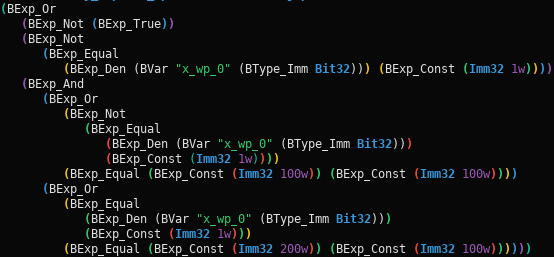
\includegraphics[width=\textwidth]{figures/test_cjmp_bir.png}
	\centering
	\caption{Auto-generated $P \implies \WP$ BIR expression for the \textit{cjmp} test.}
	\label{test_cjmp_bir}
\end{figure}

\begin{equation}
    \top \lor
    (\neg(x = 1w) \lor ((\neg(x = 1w) \lor 100w = 100w) \land (x = 1w \lor 200w = 100w)))
    \label{test_cjmp_words}
\end{equation}

\subsection{Load and store test} \label{addreq_test}

The \gls{NIC} manipulating a buffer descriptor queue, represented in BIR using memories, we need to ensure that \texttt{prove\_contract} works with programs containing memories. In this test, we will store a number $N$ in memory at address \textit{A}, then load a number into $x$ from address \textbf{B}. We want to check the following Hoare Triple: \htriple{A=B}{prog}{x=N}. Listing \ref{test_addreq_pseudocode} shows the equivalent pseudocode of the test program, Figure \ref{test_addreq_bir} the auto-generated $P \implies \WP$ expression, Figure \ref{test_addreq_words} the same expression translated in \textit{wordsTheory} and Listing \ref{test_addreq_smtlib} the auto-generated SMT-LIB 2.0 instance featuring \texttt{select} and \texttt{store} operations.

\begin{lstlisting}[
    language=C,
    backgroundcolor=\color{codebackcolour},
    commentstyle=\color{codegreen},
    keywordstyle=\color{magenta},
    stringstyle=\color{codepurple},
    label=test_addreq_pseudocode,caption=Equivalent pseudocode of the \textit{load and store} test,
    frame=tb,basicstyle=\footnotesize\ttfamily]
MEM = store(MEM, ADDR1, 42)
x = load(MEM, ADDR2)
\end{lstlisting}

\begin{figure}[!h]
	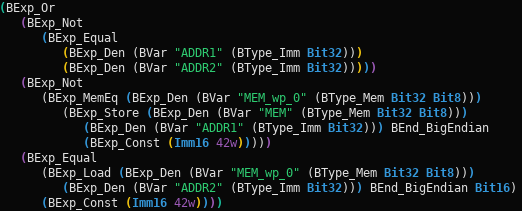
\includegraphics[width=\textwidth]{figures/test_addreq_bir.png}
	\centering
	\caption{Auto-generated $P \implies \WP$ BIR expression for the \textit{load and store} test.}
	\label{test_addreq_bir}
\end{figure}

\begin{figure}[!h]
	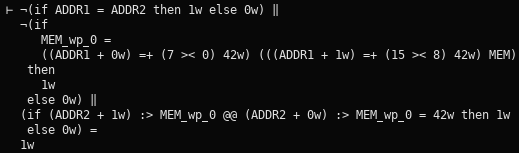
\includegraphics[width=\textwidth]{figures/test_addreq_words.png}
	\centering
	\caption{$P \implies \WP$ expression translated in \textit{wordsTheory} for the \textit{load and store} test. \texttt{><} is the bitwise extraction operation, \texttt{@@} the word concatenation operation, \texttt{|+} the memory update operation and \texttt{\textquotesingle} the memory load operation. Bit extraction and concatenation is needed because we are working with 16-bit words in a 8-bit memory.}
	\label{test_addreq_words}
\end{figure}

\begin{lstlisting}[
    language={},
    backgroundcolor=\color{codebackcolour},
    commentstyle=\color{codegreen},
    keywordstyle=\color{magenta},
    stringstyle=\color{codepurple},
    label=test_addreq_smtlib,caption=Autogenerated SMT instance for the \textit{load and store} test,
    frame=tb,basicstyle=\footnotesize\ttfamily,
    float,floatplacement=H,
    breaklines=true,postbreak=\mbox{\textcolor{red}{$\hookrightarrow$}\space}]
(set-info :source |Automatically generated from HOL4 by SmtLib.goal_to_SmtLib.
Copyright (c) 2011 Tjark Weber. All rights reserved.|)
(set-info :smt-lib-version 2.0)
(declare-fun v0_ADDR1 () (_ BitVec 32))
(declare-fun v1_ADDR2 () (_ BitVec 32))
(declare-fun v2_MEM_wp_0 ()
  (Array (_ BitVec 32) (_ BitVec 8)))
(declare-fun v3_MEM ()
  (Array (_ BitVec 32) (_ BitVec 8)))
(assert
 (not
  (=
   (bvor
    (bvnot (ite (= v0_ADDR1 v1_ADDR2)
                (_ bv1 1) (_ bv0 1)))
    (bvor
     (bvnot
      (ite
       (= v2_MEM_wp_0
        (store
         (store
          v3_MEM
          (bvadd v0_ADDR1 (_ bv1 32))
          ((_ zero_extend 0) ((_ extract 15 8) (_ bv42 16))))
         (bvadd v0_ADDR1 (_ bv0 32))
         ((_ zero_extend 0) ((_ extract 7 0) (_ bv42 16)))))
       (_ bv1 1)
       (_ bv0 1)))
     (ite
      (=
       (concat
        (select v2_MEM_wp_0 (bvadd v1_ADDR2 (_ bv1 32)))
        (select v2_MEM_wp_0 (bvadd v1_ADDR2 (_ bv0 32))))
       (_ bv42 16))
      (_ bv1 1)
      (_ bv0 1))))
   (_ bv1 1))))
(check-sat)
(exit)
\end{lstlisting}

This expression is harder to prove manually. However, SMT solvers can report very efficiently that the negated expression is unsatisfiable, proving the contract. Therefore, we see that contracts involving BIR memories can be proved, thanks to the work of Section \ref{bir-memories-with-smt-solvers}.

Other preconditions have been tested to verify that \texttt{prove\_contract} doesn't prove false contracts and succeeds to prove true ones. With the current program, the precondition $load(MEM,B=N) \land B=A+2$ can establish the postcondition. The second conjunct is important because $N$ is stored in two consecutive 8-bit memory locations. Interestingly, the precondition $\bot$ works for all contracts, because $\forall x.~\bot \implies x$, and it works in this particular case.

% TODO? \subsubsection{Gauss}
% If yes, change "two" to "three" in the subsection intro

\section{Simple automatized proofs on the NIC model}

\textbf{TODO}: In Chapter \ref{nic-model} we implemented parts of the NIC model using BIR.
+ Prove invariants
+ say that we cannot prove everything that we need
+ conclude on this chapter

\chapter{Trustful analysis on the NIC model} \label{trustful-nic-analysis}
\vspace{-1cm}
\textit{In the previous chapter, we implemented an automated non \gls{proof-producing} contract verification library, the non proof-producing part being the translation from BIR expressions to the equivalent \textit{wordsTheory} and \textit{combinTheory} expression. Moreover, this verification library can only produce contracts on BIR programs. In order to perform trustworthy verification on the \gls{NIC} model, we need to make proofs directly on the \gls{NIC} state. In this chapter, we will perform a proof on a BIR program and then lift it to the \gls{NIC} model.}

%bisimulation and lifting are recurring ideas in trustful binary verification.

In order to prove the feasibility of this approach, we will prove a simple property. Listing \ref{proof_nic_state} contains the NIC state on which we want to prove a property, Equations \ref{proof_nic_P_def}, \ref{proof_nic_Q_def} and \ref{proof_goal} present the property that we want to prove, and Listing \ref{proof_prog} contains a pseudocode representation of the BIR program on which we will perform the verification. Figure \ref{proof_schema} represents visually the structure of the verification and the steps that we will take during the proof. 

\begin{lstlisting}[
    language={},
    backgroundcolor=\color{codebackcolour},
    commentstyle=\color{codegreen},
    keywordstyle=\color{magenta},
    stringstyle=\color{codepurple},
    label=proof_nic_state,caption=NIC state used in this proof,
    frame=tb,basicstyle=\footnotesize\ttfamily]
Datatype `nic_state = <|
  dead : bool;
  x : word32
|>`
\end{lstlisting}

\begin{small}
\begin{align}
\label{proof_nic_P_def}
\vdash~&\forall nic.~P_{NIC}~nic \eqdef \neg nic.dead \land nic.x = 0w\\
%
\label{proof_nic_Q_def}
\vdash~&\forall nic~nic'.~Q_{NIC}~nic~nic' \eqdef \neg nic'.dead \land nic'.x = nic.x + 1w\\
%
\label{proof_goal}
\vdash~&\forall nic~nic'.~P_{NIC}~nic~\land~exec\_prog~nic~bir\_prog~nic'~\implies~Q_{NIC}~nic~nic'
\end{align}
\end{small}

\begin{lstlisting}[
    language=C,
    backgroundcolor=\color{codebackcolour},
    commentstyle=\color{codegreen},
    keywordstyle=\color{magenta},
    stringstyle=\color{codepurple},
    label=proof_prog,caption=Pseudocode of the program used in this proof,
    frame=tb,basicstyle=\footnotesize\ttfamily]
nic.x := nic.x + 1
if nic.x > 10:
    nic.dead := true
\end{lstlisting}

\begin{figure}[!h]
	\includegraphics[height=5cm]{figures/proof_schema.png}
	\centering
	\caption{Visual structure of the proof. References like (a) to the arrows of this Figure are used throughout the proof to refer to a particular step.}
	\label{proof_schema}
\end{figure}

%We recognize in Equation \ref{proof_goal} the equation of a Hoare Triple:
%\htriple{P(nic)}{bir\_prog}{Q(nic,nic')}.
%As already discussed \todo{make sure it is} in Section \ref{nic-model}, this structure is very common in the base lemmas of the existing proof on the \gls{NIC} model.
%However, the particularity of this Hoare Triple is that the postcondition is a function of both the initial and the final state. With the library of the previous section, postconditions involving both states are possible but involve the introduction of ghost variables.

\begin{remark} \label{remark_Q_nic_intial_final}
$Q_{NIC}~nic~nic'$ is defined on both initial and final states, in order to be able to reason about the initial state in the postcondition. This allows us to write $nic'.x = nic.x + 1w$ instead of $nic'.x = 1w$ for example.
\end{remark}

Equation \ref{proof_goal} uses a relation $exec\_prog$ that we shall define now. As we want to make a proof on an undefined HOL4 definition (a), we must establish an equivalence between the HOL4 definition (a) and the BIR program (c). In real proofs, this can either be produced by a lifter which generates the BIR program from a given input program and gives a ``certificate'', i.e. a theorem stating the equivalence, or be a definition which would then mean that we trust that the BIR program is equivalent to the HOL4 definition. In this proof, we will to use a definition. This definition shall state that $exec\_prog~nic~bir\_prog~nic'$ (a) is equivalent to executing the BIR program from a state $bir\_state$ to a state $bir\_state'$ (c), where $nic$ is somehow equivalent to $bir\_state$ (b) and $nic'$ somehow equivalent to $bir\_state'$ (d). To express an equivalence between HOL4 states ("NIC") and BIR states, we introduce a relation $R$. The relation $R~nic~bir\_state$ is defined as a simple mapping between the BIR state and the NIC state, as shown in Listing \ref{proof_R_def}. Then, we define the relation $exec\_prog$ as shown in Equation \ref{proof_eq_thm}\footnotemark.

\footnotetext{Definition \ref{proof_eq_thm} has been annotated to visualize how it is connected to the structure of the proof on Figure \ref{proof_schema}. In addition, the $BIR\_exec$ relation is used as a shorthand for $bir\_exec\_to\_labels$ in order to simplify the proof.}

\begin{lstlisting}[
    language=C,
    backgroundcolor=\color{codebackcolour},
    commentstyle=\color{codegreen},
    keywordstyle=\color{magenta},
    stringstyle=\color{codepurple},
    label=proof_R_def,caption=Definition of the relation $R$,
    frame=tb,basicstyle=\footnotesize\ttfamily]
val R_def = Define `
  R (nic: nic_state) (bir_state: bir_state_t) <=>
       (bir_env_lookup "nic_dead" bir_state.bst_environ
          = SOME (BType_Bool,
                  SOME (BVal_Imm (Imm1 nic.dead))))
    /\ (bir_env_lookup "nic_x" bir_state.bst_environ
          = SOME (BType_Imm Bit32,
                  SOME (BVal_Imm (Imm32 nic.x))))`
\end{lstlisting}

\begin{small}
\begin{equation}
\begin{split}
  \vdash \forall nic~nic'. &~exec\_prog~nic~bir\_prog~nic' ~~~~~~~~~~~~~~~~~~~~~~~~~~~~~~~~~~ \text{(a)}\\
    \eqdef~&\forall bir\_state~bir\_state'.\\
          & ~~~~~~ (R~nic~bir\_state ~~~~~~~~~~~~~~~~~~~~~~~~~~~~~~~~~~~~~~~~~~~~~~~~~ \text{(b)}\\
          & ~~~~~~ \land bir\_state' = BIR\_exec~prog~bir\_state) ~~~~~ \text{(c)}\\
          & ~~~~~~ \implies R~nic'~bir\_state' ~~~~~~~~~~~~~~~~~~~~~~~~~~~~~~~~~~~~~~ \text{(d)}
\end{split}
\label{proof_eq_thm}
\end{equation}
\end{small}

\begin{proof}[Proof of Equation \ref{proof_goal}]

\numberwithin{equation}{theorem} % Changes numbering of equations inside theorems

%\textit{\textbf{Note}: The proof has been simplified in order to focus on its global structure.}

In order to begin the proof, as the goal \ref{proof_goal} is defined over $nic$ states, we need a theorem about the injectivity of the relation $R$, stating that for all $nic$ exists a $bir\_state$ such that $R~nic~bir\_state$ (b). Additionally, the $BIR\_exec$ relation will also need some properties on $bir\_state$, that we shall add in this injectivity theorem now.

\begin{theorem} \label{proof_R_inj_thm}
Injectivity theorem of $R$
\begin{equation*} \label{proof_R_inj_thm_eq}
\begin{split}
    \vdash~\forall nic.&~\exists bir\_state.\\
    		&~~~~~R~nic~bir\_state\\
		&\land~bir\_state.bst\_pc.bpc\_index = 0\\
		&\land~bir\_state.bst\_pc.bpc\_label = entry\_label\\
		&\land~bir\_state.bst\_status = BST\_Running
\end{split}
\end{equation*}
\end{theorem}

\begin{proof}
After rewriting the relation $R$, we prove theorem \ref{proof_R_inj_thm} by exhibiting a satisfying $bir\_state$.
\end{proof}

In possession of a $bir\_state$ in relation with a $nic$, we now need to lift the precondition $P_{NIC} nic$ on this $bir\_state$. First, we need to introduce equivalent pre- ---and post- ---conditions on the BIR states, then we shall prove that the precondition lifts.

\begin{lstlisting}[
    language=C,
    backgroundcolor=\color{codebackcolour},
    commentstyle=\color{codegreen},
    keywordstyle=\color{magenta},
    stringstyle=\color{codepurple},
    label=proof_bir_conditions,caption=Equivalent pre- and postconditions on BIR states,
    frame=tb,basicstyle=\footnotesize\ttfamily]
val BIR_P_exp_def = Define `BIR_P_exp = ^(bandl [
  beq ((bden o bvarimm1) "nic_dead", bfalse),
  beq ((bden o bvarimm32) "nic_x", bconst32 0)
])`
val BIR_Q_exp_def = Define `BIR_Q_exp = ^(bandl [
  beq ((bden o bvarimm1) "nic_dead", bfalse),
  beq ((bden o bvarimm32) "nic_x", bconst32 1)
])`
val BIR_P_def = Define `BIR_P bstate =
  bir_eval_bool_exp BIR_P_exp bstate.bst_environ`
val BIR_Q_def = Define `BIR_Q bstate =
  bir_eval_bool_exp BIR_Q_exp bstate.bst_environ`
\end{lstlisting}

\paragraph{Limitation} $Q_{BIR}$ is a function of the end state only. Hence, in order to reason about the initial state in the we need in general to introduce ghost variables postcondition. In this proof, since the contract that we are proving is simple, using the actual value of $nic.x$ is enough. However, as we will discuss later on \todo{Make sure this is discussed}, this may pose a problem if we want to generalize the proof.

\paragraph{Notation} $P_{BIR}~bir\_state$ and $Q_{BIR}~bir\_state$ are defined using $bir\_eval\_bool\_exp$, which evaluates respectivelly the expressions $P^{exp}_{BIR}$ and $Q^{exp}_{BIR}$ in a given BIR state. In order to simplify the proof, let's define a new operator $\eqeval$ that is used to evaluate given variables, e.g. $bir\_state.x \eqeval 0w$.
\bigskip

\begin{theorem} \label{proof_b_thm}
Lifting of $P_{NIC}~nic$ to $bir\_state$
\begin{equation*} \label{proof_b_thm_eq}
\begin{split}
\vdash~\forall bir\_state~(\exists nic.~R~nic~bir\_state~\land~P_{NIC}~nic) \implies P_{BIR}~bir\_state
%⊢ ∀bir_state. (∃nic. R nic bir_state ∧ NIC_P nic) ⇒ BIR_P bir_state
\end{split}
\end{equation*}
\end{theorem}

\begin{proof}
Let's do this proof in a backward way. By discharging the antecedent of the implication and using the existancial elimination inference rule, we get as assumptions $P_{NIC}~nic$ and $R~nic~bir\_state$. From this, we can deduce that $bir\_state.x \eqeval 1w$ and $bir\_state.dead \eqeval \bot$. Then, we can substitute those values in the goal, which proves it.
\end{proof}

Assuming that we have a Hoare Triple theorem between initial and final BIR states, we can use Definition \ref{proof_eq_thm} in order to establish that $R~nic'~bir\_state'$. Then, in order to prove $Q_{NIC}~nic$ (d), we have to transfer the postcondition back from $bir\_state$ to $nic$.

\begin{theorem} \label{proof_d_thm}
Lowering $Q_{BIR}~bir\_state$ to $nic$.
\begin{equation*} \label{proof_d_thm_eq}
\begin{split}
\vdash~\forall~&bir\_state'.~Q_{BIR}~bir\_state' \implies\\
	&(\forall nic~nic'~bir\_state.~P_{BIR}~bir\_state\\
	&~~~~~~\land~R~nic~bir\_state~\land~R~nic'~bir\_state'\\
	&~~~\implies Q_{NIC}~nic~nic')
\end{split}
\end{equation*}
We introduce $bir\_state$ and $P_{BIR}$ in this theorem for the reason explained in Remark \ref{remark_Q_nic_intial_final}, i.e. reason about both the initial and final state in the postcondition.
\end{theorem}

\begin{proof}
This proof has been done in HOL4. The reasoning is quite similar to the proof of Theorem \ref{proof_b_thm}, as the backward proof mainly involves rewriting and simplification. We will omit this proof here and redirect the reader to the HOL4 proof available in our source repository \cite{lacroix_trustful_2019}.
\end{proof}

We will now prove that the Hoare Triple holds on the BIR program.
\bigskip

\begin{theorem} \label{proof_ht_thm}
\htriple{P^{exp}_{BIR}}{bir\_prog}{Q^{exp}_{BIR}}
\end{theorem}

\begin{proof}
To prove this Hoare Triple, we used the proof-producing procedure implemented in \gls{holba} in order to generate the weakest precondition. The automatically derived weakest precondition is shown in Figure \ref{proof_wp_exp}. Section \ref{contract-verif-holba} already discussed how to perform this proof: we have to prove Equation \ref{eval_pre_imp_eval_wp} with $\mathbf{wp}$ being the expression in Figure \ref{proof_wp_exp} and $\mathbf{pre}$ being $P^{exp}_{BIR}$. Because we want to use a \gls{SMT} solver, we need to turn the goal of the backward proof into a \textit{wordsTheory} expression. \textit{combinTheory} isn't needed in this case since BIR memories are not used. Equation \ref{eval_pre_imp_eval_wp} uses $bir\_eval\_exp$ which evaluates an expression in the given BIR state. Therefore, to translate the goal into a \textit{wordsTheory} expression, we need to use BIR's semantic. The semantic needs well-typedness and initialization of the variables. At the time of writing, HolBA offers no support for automatic rewriting with the semantic definitions, so multiple lemmas about initialization, well-typedness and type equality must be manually proved for every variable. Those are not shown here because they consist of simple rewriting and simplification.

\begin{figure}[!h]
	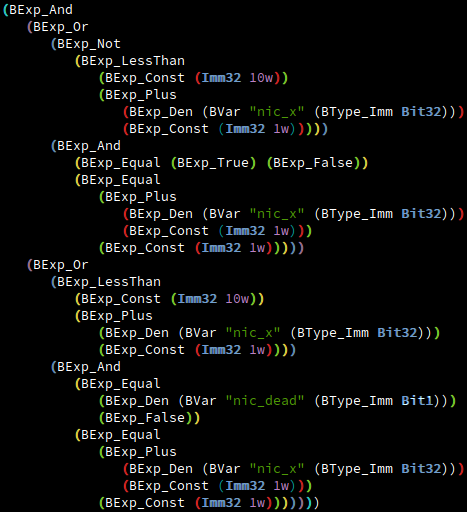
\includegraphics[scale=.65]{figures/proof_wp_exp.png}
	\centering
	\caption{Autogenerated weakest precondition for proof of Theorem \ref{proof_ht_thm}.}
	\label{proof_wp_exp}
\end{figure}

Then, the proof consist of consecutivelly rewriting following the definition of $bir\_eval\_exp$ and the definition it uses until the goal only contains $$bir\_env\_read~(BVar~``nic\_x"~(BType\_Imm~Bit32))~bir\_state.bst\_environ$$ and similarly for $nic.dead$. Let's call those expressions $x\_val$ and $dead\_val$ respectivelly. For expressions, BIR semantic is defined over immutable and constant values. Therefore, we need to establish an equivalence between the values that we currently have.

\begin{lemma}
	\begin{equation*}
		\exists x\_imm.~x\_val = BVal\_Imm~x\_imm
	\end{equation*}
	\label{proof_exists_x_imm}
\end{lemma}
\begin{proof}
Assuming well-typedness and initialization, this theorem immediately results from the BIR semantic.
\end{proof}

\begin{lemma}
	\begin{equation*}
		\exists x\_word.~x\_imm = Imm32~x\_word
	\end{equation*}
	\label{proof_exists_x_word}
\end{lemma}
\begin{proof}
This lemma is part of the BIR semantic, as one of the six conjuncts of the \texttt{bir\_imm\_t\_nchotomy} theorem, which establishes this existence theorem for every BIR immutable types.
\end{proof}

Now, using Lemma \ref{proof_exists_x_imm}, we are able to substitute all occurences of $x\_val$ into $BVal\_Imm~(Imm32~x\_word)$, and similarly for $dead\_val$. Finally, rewriting the goal using the full set of BIR semantic theorems and some rewriting rules, the goal reduces to an expression free of BIR terms:

\begin{equation} \label{proof_wp_word_goal}
\begin{split}
&(dead\_w = 0w) \land (x\_w = 0w) \implies\\
&\Big(\neg(10w <_{+} x\_w + 1w) \lor \big((1w = 0w) \land (x\_w + 1w = 1w)\big)\Big)~\land\\
&\Big((10w <_{+} x\_w + 1w) \lor \big((dead\_w = 0w) \land (x\_w + 1w = 1w)\big)\Big)
\end{split}
\end{equation}

An \gls{SMT} solver is able to prove this goal. Interrestingly, HOL4 simplification procedure are also able to prove it. However, they won't be able to prove it for more complicated ones, or will be less effective than SMT solvers.
\end{proof} % End of Hoare Triple proof

Finally, using the deduction rule with Theorems \ref{proof_R_inj_thm}, \ref{proof_b_thm}, \ref{proof_R_def}, \ref{proof_ht_thm}, \ref{proof_eq_thm} and \ref{proof_d_thm}, in that order, concludes this proof.
\renewcommand\qedsymbol{$\blacksquare$}
\end{proof}

\chapter{Conclusions}
\section{Results}

% How to evaluate the work?

\section{Discussion}

Pretty-printer, some work left:

\begin{itemize}
    \item not parsable yet
    \item no infix operators
    \item should change color of types (blue = free vars)
\end{itemize}

One-button proofs:

\begin{itemize}
    \item in binary verification, we work with ASM instead of clean C code. Therefore, pre-postconditions are harder to define. Hence, this one-button solution would need more support to easily define those expressions.
    \item prove\_contract should take definitions instead of terms for P and Q
    \item gives access to lower level functions (generate wp and simp), so it is still possible to get some control either when the proof doesn't work or if we need to use them for other tasks and compose them differently
    \item current limitations of the non pp lib: only simple linear programs; non pp; non composition;
\end{itemize}

Mention the "future" meeting that we had on the 29/05/2019.

Sound satisfiability solver for bitvectors to check if the precondition entails the weakest precondition -> same for arrays:

\begin{itemize}
    \item B ohme,  S.,  Fox,  A.C.,  Sewell,  T.,  Weber,  T.:  Reconstruction  of  Z3's  Bit-VectorProofs in HOL4 and Isabelle/HOL. In: Certified Programs and Proofs: First Inter-national Conference. pp. 183--198. Springer (2011)
    \item https://arxiv.org/pdf/1807.10664.pdf
\end{itemize}

Proof: automate (???; semantic rewriting (i.e. automatically add all the lemmas) (il faut d'abord tester à la main avant d'implémenter des procédures automatiques))

\section{Future work}

\printbibliography[heading=bibintoc]

\appendix

\chapter{LogLib's design} \label{annex_loglib}

Reference in Section \ref{impl_convenient_ht_interface}, but the need arised in general when debugging HOL4 code for tracing code (we can leave trace functions using LogLib and define different levels of verbosity).

Introduce tracing in HOL4 in general

\chapter{DepGraph's design} \label{annex_depgraph}

\tailmatter % back cover page

\end{document}
